%#! platex 000main.tex
\chapter{提案手法}
  \label{sec:method}
  エッジ抽出を行った画像から線の経路を求める. できるだけヒトが描いたような描き順になるようにするために、まず実際にこの絵を自分が描いたときの描き順を調べた. 右利きと仮定すると、左側から描き始めることが多かった. そのため、本研究ではスタートを頭部の輪郭の左側から描けるようにした. そのためにある領域を端点を用意する.
  \section{描き順の分析}
  \label{sec:analysis }
  私は顔の輪郭から始まり首や目、鼻などの細部へと移って描いていく. これは全体から細部へと移ることで、パーツの位置を決めやすい体と考えられる. また右利きの場合、スタートは左側から描いていた. 理由は右利きの場合、ペンを右に傾けて持つため時計周りに円を描くほうが描きやすいからだと考えられる. 半時計周りの場合、6時から12時までの区間を描くには手を少し持ち上げて描く必要があるため、寝かせたまま描ける時計周りより不安定になる.
	\section{領域と端点を用いた経路の求め方}
    \label{sec:the way of the route}
	\subsection{スタート地点の決め方}
	\label{sec:how to define the start point}
	スタート位置を決めるためにある大きさの領域を用意した. 領域は左上の位置が横全体の$\frac{1}{8}$、縦全体の$\frac{1}{3}$、サイズが全体の$\frac{1}{4}$になるように設定した. このように領域の位置とサイズを定義することで、頭部の左側に領域が被るように設定することができた. 領域が頭部の左側にあるかを2つの画像で確かめた. 図4.1の左が''金髪女の横顔``、右が''若い女の横顔``という作品である. 以下にその例を示す. 
	  \begin{center}
        \begin{figure}[h]
            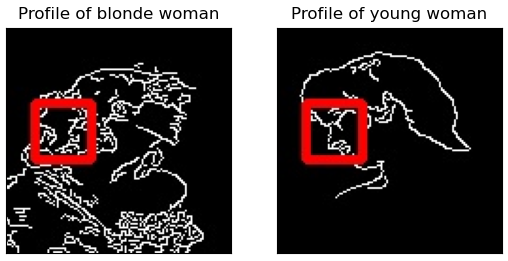
\includegraphics[width=0.90\textwidth]{/home/morita/ros2_ws/Memo/tex/img/003.png}
            \caption{領域の位置の確認}
            \label{the position of a region}
        \end{figure}
    \end{center}
	この領域を縦方向にスキャンし、最初にエッジの画素にぶつかった位置をスタート地点に決める.
	\subsection{端点の検出と線の辿り方}
	\label{chap:end points detection}
	図4.1ではエッジが綺麗に繋がっているように見えるが、拡大すると途切れている. そのため、ロボットにそのままエッジの画素をそのまま座標として与えると実際の線画が点線になってしまう. そこで端点を用いる. 線の画素を辿り、端点まで来たら次に近くの端点へ移動して描いていく. この処理を行うことで実際には点線を描くことになるが、擬似的に線を描いていくような動作ができる.
	線の辿り方はある線の画素から隣に線の画素があるかを探し、線の画素があれば移動し、なければ最も近いまだ通過していない端点へと移動する. これを線の画素がなくなるまで繰りかえす.

